%*******************************************************************************
%****************************** Appendix B *************************************
%*******************************************************************************
		\chapter{Equipment} \label{appendix:b}

%% **************************** Define Graphics Path **************************
%\ifpdf
%    \graphicspath{{appendixB/figs/raster/}{appendixB/figs/PDF/}{appendixA/figs/}}
%\else
%    \graphicspath{{appendixB/figs/vector/}{appendixB/figs/}}
%\fi


\graphicspath{{figs/appendixB/PDF/}}

%
%\appendix
%\hypertarget{aA}{ \section*{Appendix B. Inertial Sensors}}  \label{appendix:b}
%


\section{NeMEMsi IMU sensors}  \label{appendix:imus}
For this work, data were collected using NeMEMsi sensors \cite{Comotti2014}
that provide 3D accelerometer, 3D magnetometer, 3D gyroscope and quaternions
(Figure~\ref{fig:muse}).
It is important to note that NeMEMsi sensors 
were tested against the state-of-the-art device MTi-30 IMU from xsense.
The comparison values between NeMEMsi and MTi-30 in terms of standard deviation 
of the noise of each component of the Euler angles at a state state are lower than
0.1 degrees. 
Additionally, the NeMEMsi provide not only to have a lower-power consumption 
but also the smaller dimensions againts other state-of-the-art brands of IMUs.

In the following sections, some features of the IMU are presented,
however, we refer the readers to check \cite{Comotti2014} for further details.

\subsection*{Sample rate and power consumption}
Data streaming can be set up to be streamed at 25 Hz, 50 Hz and 100Hz which
affects the power comsuption from 29mAh, 32mAh and 35mAh, respectively.
For this work, the sample rate were set up to 50 Hz.

\subsection*{Sensors}
The outputs of the NeMEMsi sensor include:

\subsubsection*{Orientation}
* Euler angles (Yaw, Pitch and Roll).
* Quaternions.

\subsubsection*{Accelerometer (Linear acceleration)}
* Raw and calibrated XYZ measurement from $\pm$2 / $\pm$4 / $\pm$6 / $\pm$8  / $\pm$16

\subsubsection*{Gyroscope (Rate of turn)}
* Raw and calibrated XYZ measurement from $\pm$245 /  $\pm$500 / $\pm$2000 degrees per second.

\subsubsection*{Magnetometer (Magnetic field)}
* Raw and calibrated XYZ measurement from $\pm$4 / $\pm$8 / $\pm$12 / $\pm$16 gauss.


\subsection*{Microprocessor}
* Arquitecture: ARM 32-bit Cortex M4 CPU with FPU and DSP instructions
* Max.frequency: 100MHz
* Memory Size: 512 Kbytes
* RAM: 128 Kbytes SRAM


\subsection*{Connectivity}
* Bluetooth: Class 2, bluetooth 3.0
* Range: 10 m
* Transmission rate: Up to 560 kbps with Service Port to Port
* Multipoint: Up to 7 slaves


\subsection*{Form factor}
* Electronics physical dimension: 25L x 25W x 4H (mm)
* Electronics Weight: 3.3 gr
* Dimension with battery and casing: 42L x 28W x 11.5 (mm)
* Weight with batter and casing: 15 gr


%%---------------------------------(FIGURE)-------------------------------------
\begin{figure}
 \centering
   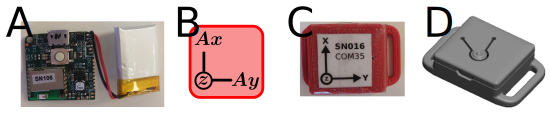
\includegraphics[width=1.0\textwidth]{muse}
   \caption{Inertial Measurament Sensor:
		(A) Printed Circuit Board (PCB) with 165mAh battery,
		(B) axis orientation, 
		(C) real case, and 
		(D) 3D model for the case.
}
   \label{fig:muse}
\end{figure}
%%---------------------------------(FIGURE)-------------------------------------

\section{Time-series preprocessing}
\subsection{Organising Data in Multidimensional Arrays}

Scripts in \MATLAB were created to syncronise the data using the clock drift and clock
offset values which were provided for each of the NeMEMSi sensors.
Then the data from each sensor is aligned in time using using
\texttt{finddelay()} and \texttt{alignsignals()} in \MATLAB.

The use of \texttt{alignsignals()} is useful when the data is relatively clean
that means that when data was noisy the alignment were not even close
when two signals were quite similar. Therefore, I decided to
program my own \texttt{alignsignalsMX()} to use the synchronised
data but with different length.


Scripts in \R  were used for postprocessing the data.

\subsection{Data Synchornisation}

To find the delay between two two sensors that were attached to the same place
of the body parts, a function called  \texttt{finddelayMX()} was created.
Such function computes the autocorrelation between two signals using \texttt(xcorr())
then the maximum value of the the autocorrleation function is extracted
to create a delay between the values of maximum index in the autocorrelation
function and the length of the first signal

% [R, lag] = xcorr(X,Y);
% [Y,I] = max(R);  %%%[Y,I] = max(X) returns the indices of the maximum values in vector I.
% delay = abs(I - length( X ) );

The function \texttt{alignsignalsMX()} was used to align two signals based
on \texttt{finddelayMX()}. The function \texttt{alignsignalsMX()} use six inputs
of which sA and sB are the sensors, then the windowframe of which the information
of the signal is extracted from another activities, the MainAxis of which the
signal are going to be extracted, the truncate delay that is created to
syncrohnise the signals adding an extra delay that is based on the lenght of
previous signals and tunning delay that can be useful to tune the delay in the
case of the dalay is not appropriate when the signals are too noisy.
% function [a,b,delay] =
% alignsignalsMX(sA,sB,windowframe,MainAxis,truncate_delay, tuning_delay)

Then, it is used the \texttt{aligntwosignals()} to align only two signals.
The inputs of \texttt{aligntwosignals()} are X and Y for the input vectors,
truncate delay for the previous delay of two signals and tunning delay
in case that signals are two noise and the xcorr fail to find an appropriate
delay.
 % function [a,b,delay] = aligntwosignals(X,Y,truncate_delay, tuning_delay)

\subsection{Time Alignment}
It was taken another approach to align the data in time in which the
original synchronised data is manipulated. Given four vectors of time
$t_1, t_2, t_3, t_4$, it is extracted the minimum and maximum values
of the start of the four sequence of time,
it was also exrtacted the minimum and maximum values to the
end of the four sequence of time.

However, after aligning the vectors it has then  been noticed that there were
different values of lenght across vectors i.e.: $1880,1986,1987,1988$
Therefore the lenght for the second vector was used as the primary lenght
becase is the one that is present the minimum value of the three maximum
lenghts. Then \texttt{interp1(x,v,vq,'phchip')}  was used to interpolate the
length of each of the vectors such as the length of all vectors is: $1986,1986,1986,1986$.
It has been choosen the \texttt{phchip} since the interpolation present
values for each of the points which were different for the NA values
from what it has been got when using \texttt{linear}.

\subsection{Issues with IMUs} \label{appendix:imus:issues}


\section{Humanoid robot}  \label{appendix:nao}
\subsection{Hardware}
\subsection{Software}



